% Drawing 154/03-12 -- folder 154, batch 03, archive page 45 (PDF page 46).
% Transcription: figures dans l'entre-colonne : une droite verte et deux traits rouge orangé se croisant en un point marqué $s$, un trait bleu gris au point de croisement, des tirets verts de part et d'autre ; au-dessous, un octogone vert en deux moitiés, $F$ et $F'$, traversé d'un faisceau rouge orangé en forme de lentille resserrée au milieu en $s$ (un petit trait bleu), les pointes marquées $t$, $t'$, $t''$, $t'''$
% Kind: crossing at s; two faces F, F' crossed by a pinched pencil. Method 2 (schematic redraw from the facsimile). Status: ok.
% Notes: Upper figure: the light green line, two strokes crossing on it at s (point computed), the blue-grey stroke across the crossing, two rows of green dashes. Lower figure: the two faces F and F' drawn as dashed light green polygons sharing a side, the pencil of three strokes fanning from s upwards into F and three downwards into F', the short blue stroke across the waist, the black point by s; t is written at the upper tips and the three primed letters below the lower tips, placed after the transcription (they are small on the page). The polygons have seven or eight sides each as read; their exact number of sides is not sure. Redrawn 2026-11-12 (issue 128): to check again. 2026-11-14, Claude Opus 5.5, overlay check (issue 147): rasterised from its own coordinates over the 400 dpi colour scan on a unit grid, corrected and laid over it again; not compiled (no TeX in the session). Upper figure: the green line lengthened to its ink at both ends; the two orange strokes moved onto their ink (the second lay up to 6 units off: it runs from (54.4,-23.9) down to (79,-33.5)); the blue-grey stroke moved onto its ink; the two rows of green dashes are one dashed curve on the page, from the green line at (59.3,-38) under the crossing and up the right side to (79.8,-20.8), drawn so. Lower figure, redrawn from a 26 px-per-unit reading: the two faces are drawn as the separate thick light green dashes the page has (seven for F, five for F', the dash at the waist shared), not as closed polygons; the three red strokes above the waist leave one point under t and fan out into a spindle that closes again at the waist (the earlier redraw fanned them from the waist to three separate points); the three below run from the waist to three separate ends above t', t'', t'''; the short blue stroke across the waist moved onto its ink. Every stroke now lies on its ink to within about 1 unit. Status set to ok.
% Coordinates: 1 unit = 1 mm = 1/100 of the crop width (bbox in page fractions: [0.575, 0.215, 0.77, 0.375]).
% Redrawn by Claude (claude-fable-5-2), issue #128, 2026-11-12; not checked by a human; not compiled (no TeX in the session).
% Checked by Claude (claude-opus-5-5) 2026-11-14 (issue #147): overlaid on the 400 dpi colour facsimile, corrected; not compiled (no TeX in the session). Not checked by a human. Status: ok.
% Rights: reproduces part of the work -- behind RENDER_TRANSCRIPTS, never published by itself.
\documentclass[tikz,border=3pt]{standalone}
\usepackage{amsmath,amssymb}
\usetikzlibrary{patterns,arrows.meta}
\tikzset{Lg/.style={green!60!black!70}, Rd/.style={red!85!black}, Bl/.style={blue!70!black}, Gy/.style={black!40}, pencil/.style={black!45}, struck/.style={black!35}, mpt/.style={circle,draw,inner sep=1.3pt}, pt/.style={circle,fill,inner sep=0.9pt}, opt/.style={circle,draw,fill=white,inner sep=1.1pt}}
\begin{document}
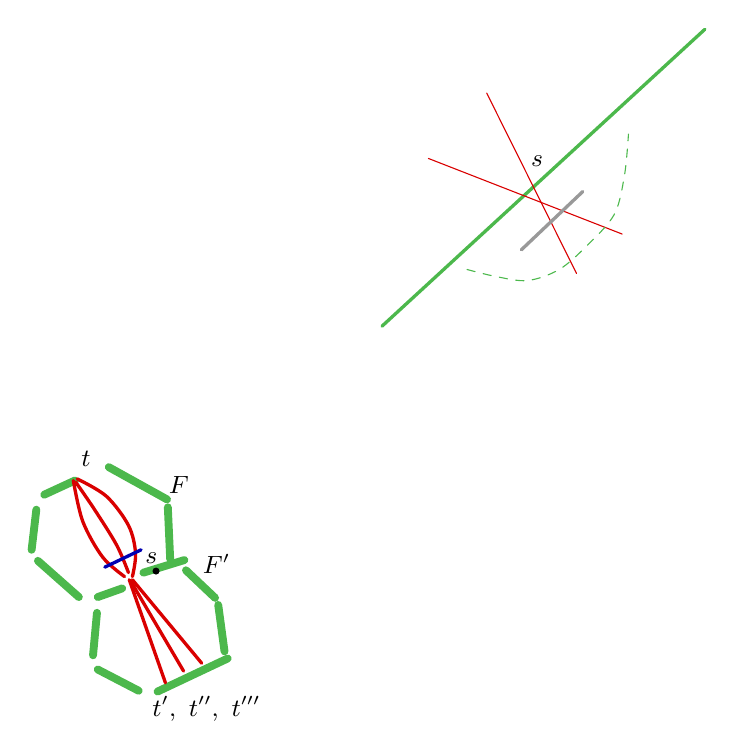
\begin{tikzpicture}[x=1mm,y=1mm,line cap=round,line join=round,font=\scriptsize]
\draw[Lg,very thick] (48.5,-45.2) -- (89.5,-7.5);
\draw[Rd] (61.8,-15.6) -- (73.2,-38.5);
\draw[Rd] (54.4,-23.9) -- (79,-33.5);
\draw[Gy,very thick] (66.2,-35.5) -- (74,-28.1);
\draw[Lg,dashed] plot[smooth, tension=0.55] coordinates {(59.3,-38) (63,-38.9) (67,-39.4) (71,-38) (74.5,-35) (78,-31) (79.3,-26) (79.8,-20.8)};
\node[inner sep=1pt] at (68.2,-24.2) {\small $s$};
\draw[Lg,line width=1mm] (5.6,-66.6) -- (9.5,-64.8);
\draw[Lg,line width=1mm] (13.8,-63.1) -- (21.2,-67.2);
\draw[Lg,line width=1mm] (21.3,-68.2) -- (21.6,-74.8);
\draw[Lg,line width=1mm] (4.6,-68.5) -- (4,-73.6);
\draw[Lg,line width=1mm] (4.8,-75) -- (10,-79.6);
\draw[Lg,line width=1mm] (12.4,-79.6) -- (15.5,-78.5);
\draw[Lg,line width=1mm] (18.2,-76.5) -- (23.4,-74.9);
\draw[Lg,line width=1mm] (12.3,-81.6) -- (11.8,-87);
\draw[Lg,line width=1mm] (12.4,-88.8) -- (17.6,-91.5);
\draw[Lg,line width=1mm] (20,-91.6) -- (28.9,-87.4);
\draw[Lg,line width=1mm] (28.5,-86.5) -- (27.7,-80.6);
\draw[Lg,line width=1mm] (23.6,-76.2) -- (27.3,-79.7);
\draw[Rd,very thick] plot[smooth, tension=0.55] coordinates {(9.3,-64.8) (10.5,-70) (13,-74.5) (15.8,-77)};
\draw[Rd,very thick] plot[smooth, tension=0.55] coordinates {(9.6,-65) (12,-68.5) (14.8,-73) (16.3,-76.5)};
\draw[Rd,very thick] plot[smooth, tension=0.55] coordinates {(9.8,-64.6) (13.5,-66.8) (16.3,-70.5) (17.2,-74) (16.8,-77)};
\draw[Rd,very thick] (16.4,-77.4) -- (21,-90.5);
\draw[Rd,very thick] (16.6,-77.6) -- (23.3,-89);
\draw[Rd,very thick] (16.8,-77.4) -- (25.6,-88);
\draw[Bl,very thick] (13.3,-75.8) -- (17.9,-73.6);
\node[pt] at (19.8,-76.3) {};
\node[inner sep=1pt] at (19.2,-74.6) {\small $s$};
\node[inner sep=1pt] at (22.7,-65.4) {\small $F$};
\node[inner sep=1pt] at (27.5,-75.4) {\small $F'$};
\node[inner sep=1pt] at (10.9,-62.1) {\small $t$};
\node[inner sep=1pt] at (26.2,-93.8) {\small $t',\ t'',\ t'''$};
\end{tikzpicture}
\end{document}
